\section{Control Cinematico del robot}
\begin{itemize}
	\item HABLAR SOBRE QUE ES EL CONTROL CINEMATICO Y LAS MOVIDAS DE LOS GENERADORES DE TRAYECTORIAS
\\Una vez estudiado el análisis cinemático del modelo de brazo manipulador, y obtenidas las ecuaciones cinemáticas inversa y directa de este, se terminará de abordar el problema cinemático, al ser capaces de desarrollar el control sobre esta; para ello, se requiere poder generar trayectorias dentro del espacio articular, con tal de que el brazo manipulador pueda cumplir una ordenes de movimiento conocidas, en este caso dadas en un espacio cartesiano.\\

\item TIPOS DE TRAYECTORIAS. COMO LA GENERAMOS
\\Visto esto, tenemos que conocer las consignas de movimiento, mejor vistas como condiciones de contorno o exigencias, que se le piden al robot; ejemplificado en este proyecto, el movimiento del efector final entre dos puntos del espacio cartesiano del robot, dado un tiempo limite para su realización.\\

	\item INTERPOLADORES DE TRAYECTORIAS
	\item IMPLEMENTACION, GRAFICAS Y CONCLUSCIONES 
\end{itemize}
	\subsection{Generador de trayectorias punto a punto}
	 
	\subsection{Generador de trayectorias lineal}
	
	\subsection{Generador de trayectorias circulares}
	El generador de trayectorias circulares es similar al generador de trayectorias lineal, excepto por el cálculo de la trayectoria en sí, es decir, una vez obtenidos los puntos que definen la trayectoria, se realizan los mismos cálculos para la obtención de las posiciones, velocidades y aceleraciones articulares.
	
	Para empezar, se deben introducir 3 puntos, a diferencia de los generadores lineales, que definirán la curva como punto inicial, punto intermedio y punto final. Lo próximo que se calcula es el centro de la circunferencia definida de tal forma:
	
	Primero se calcula el vector unitario perpendicular al plano definido por la circunferencia:
	\begin{center}
	$v_1=(P_2-P_1)\wedge(P_3-P_1)$\\
	$v_1=v_1/||v_1||$\\
	\end{center}

	Una vez obtenido dicho vector, se puede pasar al cálculo del centro de la circunferencia, lo cual se realiza con un sistema de 3 ecuaciones que se resuelve de forma matricial y que se haya buscando relaciones entre vectores (puede haber más de un sistema de ecuaciones que lleve a la resolución del problema):
	\begin{center}
		1.-El producto escalar entre el vector $v_1$ y el vector definido por $P_0-P_1$ ha de ser nulo\\
		
		2.-El producto escalar entre el vector $P_0-(P_2+P_1)/2$ y el vector $P_2-P_1$ ha de ser nulo\\
		
		3.-El producto escalar entre el vector $P_0-(P_3+P_1)/2$ y el vector $P_3-P_1$ ha de ser nulo\\
	\end{center}	
	Una vez obtenidas las ecuaciones se ha de obtener el sistema de ecuaciones tal que:\\
	\begin{center}
		$P_0=A|B$\\
	\end{center}	
	Realizando las operaciones pertinentes y despejando se pueden obtener las matrices A y B como:\\
	\begin{center}
		$$
		A=
		\begin{bmatrix}
			v_1(1) & v_1(2) & v_1(3)\\
			P_2(1)-P_1(1) & P_2(2)-P_1(2) & P_2(3)-P_1(3)\\
			P_3(1)-P_1(1) & P_3(2)-P_1(2) & P_3(3)-P_1(3)\\
		\end{bmatrix}
		$$\\
		{\small
		$$
		B=
		\begin{bmatrix}
			P_1(1)*v_1(1)+P_1(2)*v_1(2)+P_1(3)*v_1(3)\\
			((P_2(1)+P_1(1))*(P_2(1)-P_1(1)))/2+((P_2(2)+P_1(2))*(P_2(2)-P_1(2)))/2+((P_2(3)+P_1(3))*(P_2(3)-P_1(3)))/2\\
			((P_3(1)+P_1(1))*(P_3(1)-P_1(1)))/2+((P_3(2)+P_1(2))*(P_3(2)-P_1(2)))/2+((P_3(3)+P_1(3))*(P_3(3)-P_1(3)))/2\\
		\end{bmatrix}
		$$}
	\end{center}

	Una vez hallado el centro de la circunferencia, $P_0$, se debe proceder a calcular los puntos solicitados al principio del algoritmo. Para ello se necesitarán dos vectores:
	\begin{center}
		$v_2=(P_1-P_0)/||(P_1-P_0)||$ y $v_3=-(v_2 \wedge v_1)/||(v_2 \wedge v_1)||$,\\
	\end{center}
	que serán, respectivamente, el vector unitario que va desde el centro de la circunferencia al punto $P_1$ y el vector unitario perpendicular al plano definido por $v_1$ y $v_2$ con origen en $P_1$ y sentido de la trayectoria. Con estos dos vectores se pueden calcular los puntos que compondrán la trayectoria de tal forma:\\
	
	\begin{center}
		$g=(P_3-P_0)/||(P_3-P_0)||$\\
		$cos_g=(v_2 \cdot g)$\\
		$sin_g=||v_2 \wedge g||$\\
		$rhofin=2*pi-atan2(sin_g,cos_g)$\\
		$rho=linspace(0,rhofin,npuntos)$\\
		$P=repmat(P_0,1,numel(rho))+R*(v_2*cos(rho)+v_3*sin(rho))$\\
	\end{center}

	Siendo $rhofin$ el ángulo de la posición final de la trayectoria con respecto a la posición inicial, $rho$ el vector de N puntos de valores de ángulos desde 0 hasta el ángulo de la posición final, $R$ el radio del arco de circunferencia calculado como $||P_1-P_0||$, y $P$ la matriz de posiciones correspondientes a los puntos equidistantes a lo largo de la trayectoria.\\
	
	Una vez realizados estos pasos ya se puede pasar al cálculo de los valores de las variables articulares para las posiciones calculadas como se ha llevado a cabo en los generadores anteriores.\\
	
	Los resultados obtenidos para una trayectoria específica y un valor de 100 puntos a calcular han sido los siguientes:\\
	
	\begin{figure}[H]
	\centering
	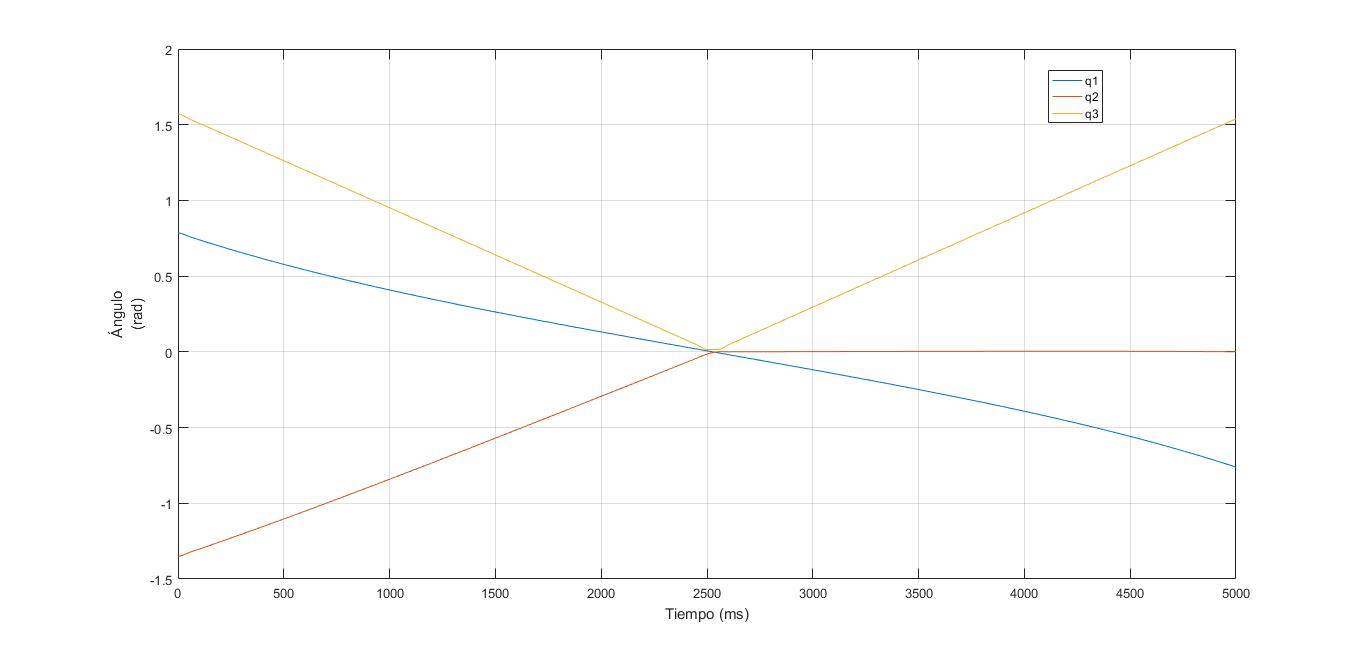
\includegraphics[width=1\textwidth]{GDT_C_articulares}
	\caption{Valores de las variables articulares}
	\end{figure}

	\begin{figure}[H]
	\centering
	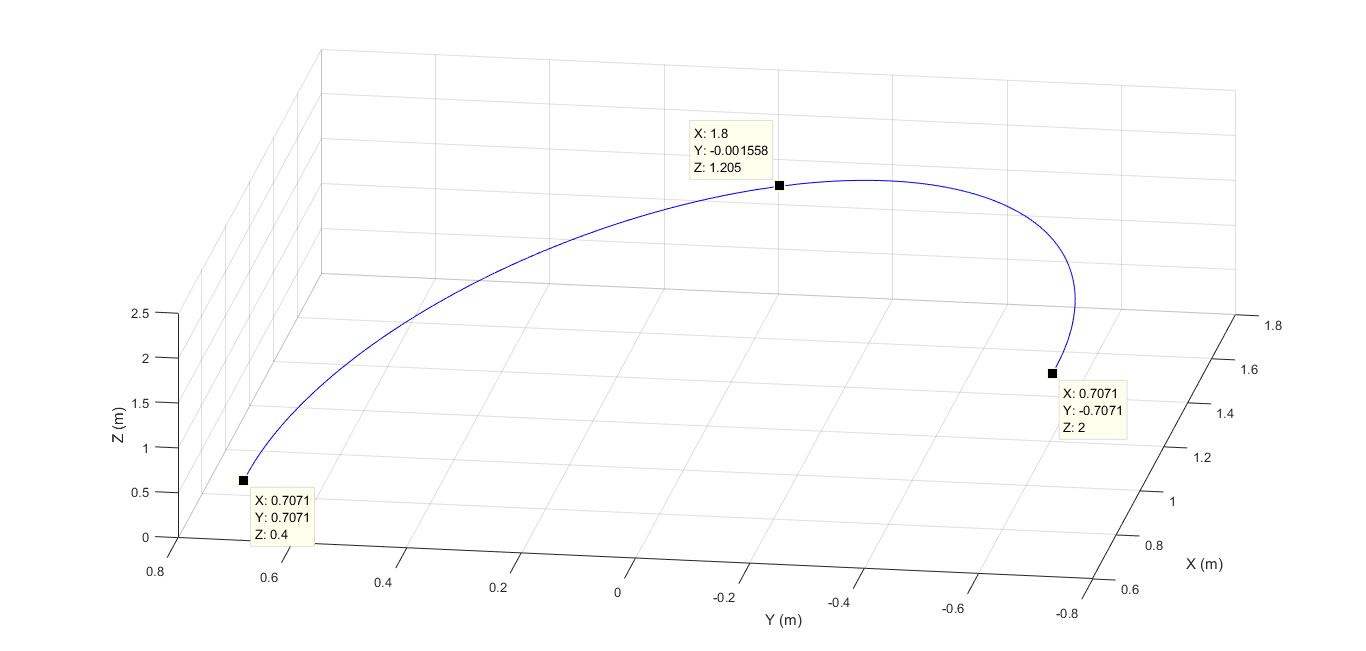
\includegraphics[width=1\textwidth]{GDT_C_efector}
	\caption{Posición del efector final}
	\end{figure}

	





	
	\subsection{Pruebas y conclusiones}
		Necesidad para el trabajo-->
		 Ser capaces de que nuestro modelo de brazo manipulador ejecute ordenes de movimientos basados en trayectorias.
		  
	    Como lo conseguimos-->
	   		Generar trayectorias de referencia en el espacio articular de nuestro modelo brazo manipulador, para conseguir